%\documentclass{article}
%\let\vec\mathbf
%\usepackage{graphicx}
%\usepackage{amsmath}
%\usepackage{gensymb}
%\usepackage{float}
%\graphicspath{{./documents/}{./figs}}
%\begin{document}
\begin{enumerate}[label=\thesection.\arabic*.,ref=\thesection.\theenumi]
\numberwithin{equation}{enumi}
\numberwithin{figure}{enumi}
\numberwithin{table}{enumi}
\item During the lockdown period, many families got bored of watching $ TV $ all the time. Out of these families, 
 one family of 6 members decided to play a card game. 17 cards numbered 1, 2, 3, 4, . . . ,17 are put in a box 
 and mixed thorougly. One card is drawn by one member at random and other family members bet for the chances 
 of drawing the number either prime, odd or even etc.
		\begin{figure}[H]
			\centering
			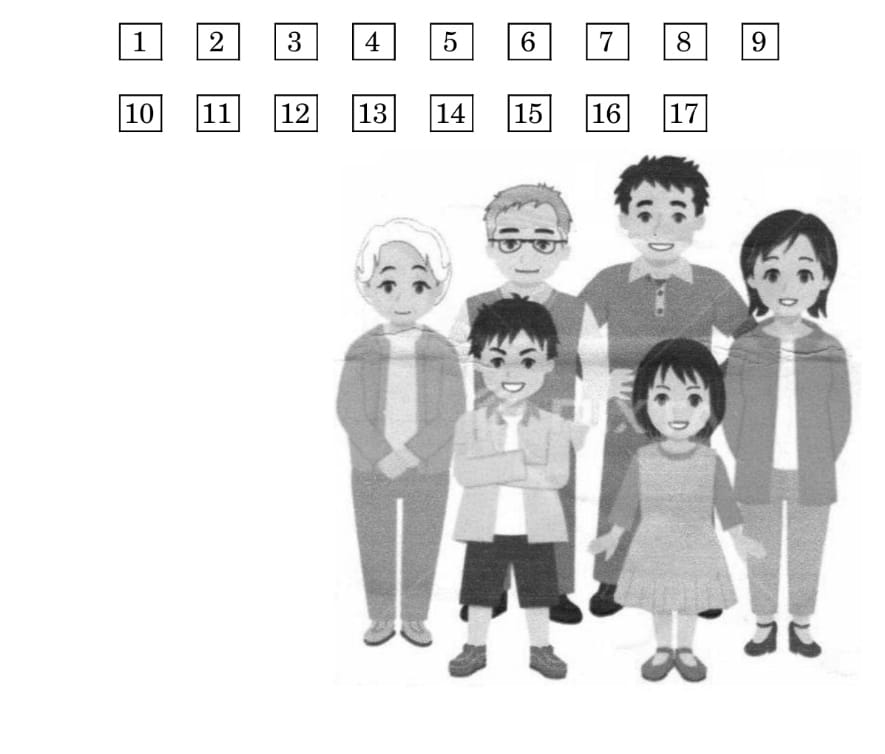
\includegraphics[width=\columnwidth]{figs/linear.jpg}
			\caption{}
			\label{fig}
		\end{figure}
		Based on thee above, answer the following questions : 
		\begin{enumerate}
			\item The first member of the family draws a card at random and another member bets that 
				it is an even prime number. What is the probability of his winning the bet ?
				\begin{enumerate}
					\item $ \frac{2}{17} $
					\item $ \frac{3}{17} $
					\item $ \frac{1}{17} $
					\item $ \frac{4}{17} $
				\end{enumerate}
			\item The second member of the family draws a card at random and some other member bets 
				that it is an even number. What is the probability of his winning the bet ? 
				\begin{enumerate}
					\item $ \frac{7}{17} $
					\item $ \frac{8}{17} $
					\item $ \frac{9}{17} $
					\item $ \frac{10}{17} $
				\end{enumerate}
			\item What is the probability that the number on the card drawn at random is divisible 
				by 5 ?
				\begin{enumerate}
					\item $ \frac{5}{17} $
					\item $ \frac{4}{17} $
					\item $ \frac{3}{17} $
					\item $ \frac{2}{17} $
				\end{enumerate}
			\item What is the probability that the number on the card drawn at random is multiple 
				of 3 ? 
				\begin{enumerate}
					\item $ \frac{5}{17} $
					\item $ \frac{6}{17} $
					\item $ \frac{7}{17} $
					\item $ \frac{8}{17} $
				\end{enumerate}
			\item What is the probability that the number on the card is a factor of 9 ?
				\begin{enumerate}
					\item $ \frac{9}{17} $
					\item $ \frac{3}{17} $
					\item $ \frac{8}{17} $
					\item $ \frac{1}{17} $
				\end{enumerate}
		\end{enumerate}
	\item If the graph of a pair of lines $ x - 2y + 3 = 0 $ and $ 2x - 4y = 5 $ be drawn, that what type of 
		lines are drawn ? 
\end{enumerate}
%\end{document}
